\documentclass{ximera}  


\input{../preamble.tex}



 
\title{Impedance and admittance circles on the Smith Chart} 
\author{Milica Markovic} 
\outcome{Explain how was Smith Chart developed.}
\begin{document}  
\begin{abstract}  

\end{abstract}  
\maketitle    





\section{Reflection Coefficient and Impedance}



Reflection coefficient and impedance are related through Equation \ref{eq:SCDereqnreflectioncoefficient}. We can find an impedance that corresponds to the reflection coefficient, Equation \ref{eq:SCDereqnimpedancerc}. Every point on the Smith Chart represents one reflection coefficient $\Gamma$ and one impedance $Z_L$. 



\begin{eqnarray}
\Gamma = \frac{Z_L-Z_\circ}{Z_L+Z_\circ} \label{eq:SCDereqnreflectioncoefficient} \\ \nonumber \\
Z_L = Z_0 \frac{ 1+ \Gamma}{1- \Gamma } \label{eq:SCDereqnimpedancerc}
\end{eqnarray}


All impedances on the Smith Chart are normalized to the transmission line impedance $Z_0$. The normalized impedance is denoted in Equation \ref{eq:SCDerNormImp} with lowercase $z_L$.

\begin{eqnarray}
z_L = \frac{Z_L}{Z_0} = \frac{ 1+ \Gamma}{1- \Gamma } \label{eq:SCDerNormImp}
\end{eqnarray}

\section{Derivation of Impedance and Admittance Circles on the Smith Chart}

Impedance and reflection coefficient are complex numbers. The normalized impedance has a real and imaginary part $z_L=r_L + j x_L$, and the reflection coefficient can also be shown in Cartesian coordinates as $\Gamma = \Gamma_r + j \Gamma_i $. We can now substitute these equations into Equation \ref{eq:SCDerRealImag}.

\begin{eqnarray}
r_L + j x_L = \frac{ 1+\Gamma_r + j \Gamma_i}{1- (\Gamma_r + j \Gamma_i)} \label{eq:SCDerRealImag}
\end{eqnarray}

We can equate the real and imaginary parts on the left and right side of Equation \ref{eq:SCDerRealImag} to get the equations of constant $r_L$ and $x_L$.


\begin{eqnarray}
\left( \Gamma_r - \frac{r_L}{1+r_L}   \right)^2 + \Gamma_i^2  =\left( \frac{1}{1+r_L}   \right) ^2 \label{eq:SCDerRealCirc} \\
\left( \Gamma_r - 1   \right)^2 + \left(\Gamma_i - \frac{1}{x_L}    \right)^2  =\left( \frac{1}{x_L}   \right) ^2 \label{eq:SCDerImagCirc}
\end{eqnarray}

These are equations of a circle, with the constant resistance  circle's center at $(\frac{r_L}{1+r_L} ,0)$ and radius $\frac{1}{1+r_L} $; and the constant reactance imaginary circle center at $(1,\frac{1}{x_L})$ and radius of $ \frac{1}{x_L}  $.

Figures \ref{fig:SCDerscresistance}- \ref{fig:SCDerscreactance}  show circles on the Smith Chart that represent constant (normalized) reactances, and resistances. 
\begin{figure}[htbp]
\begin{center}
\includegraphics[scale=0.3]{/../jpg/smithchartreal.jpg}
\end{center}
\caption{All points on the circle have the constant real part of the impedance (resistance). Normalized resistance circles.}
\label{fig:SCDerscresistance}
\end{figure}


\begin{figure}[htbp]
\begin{center}
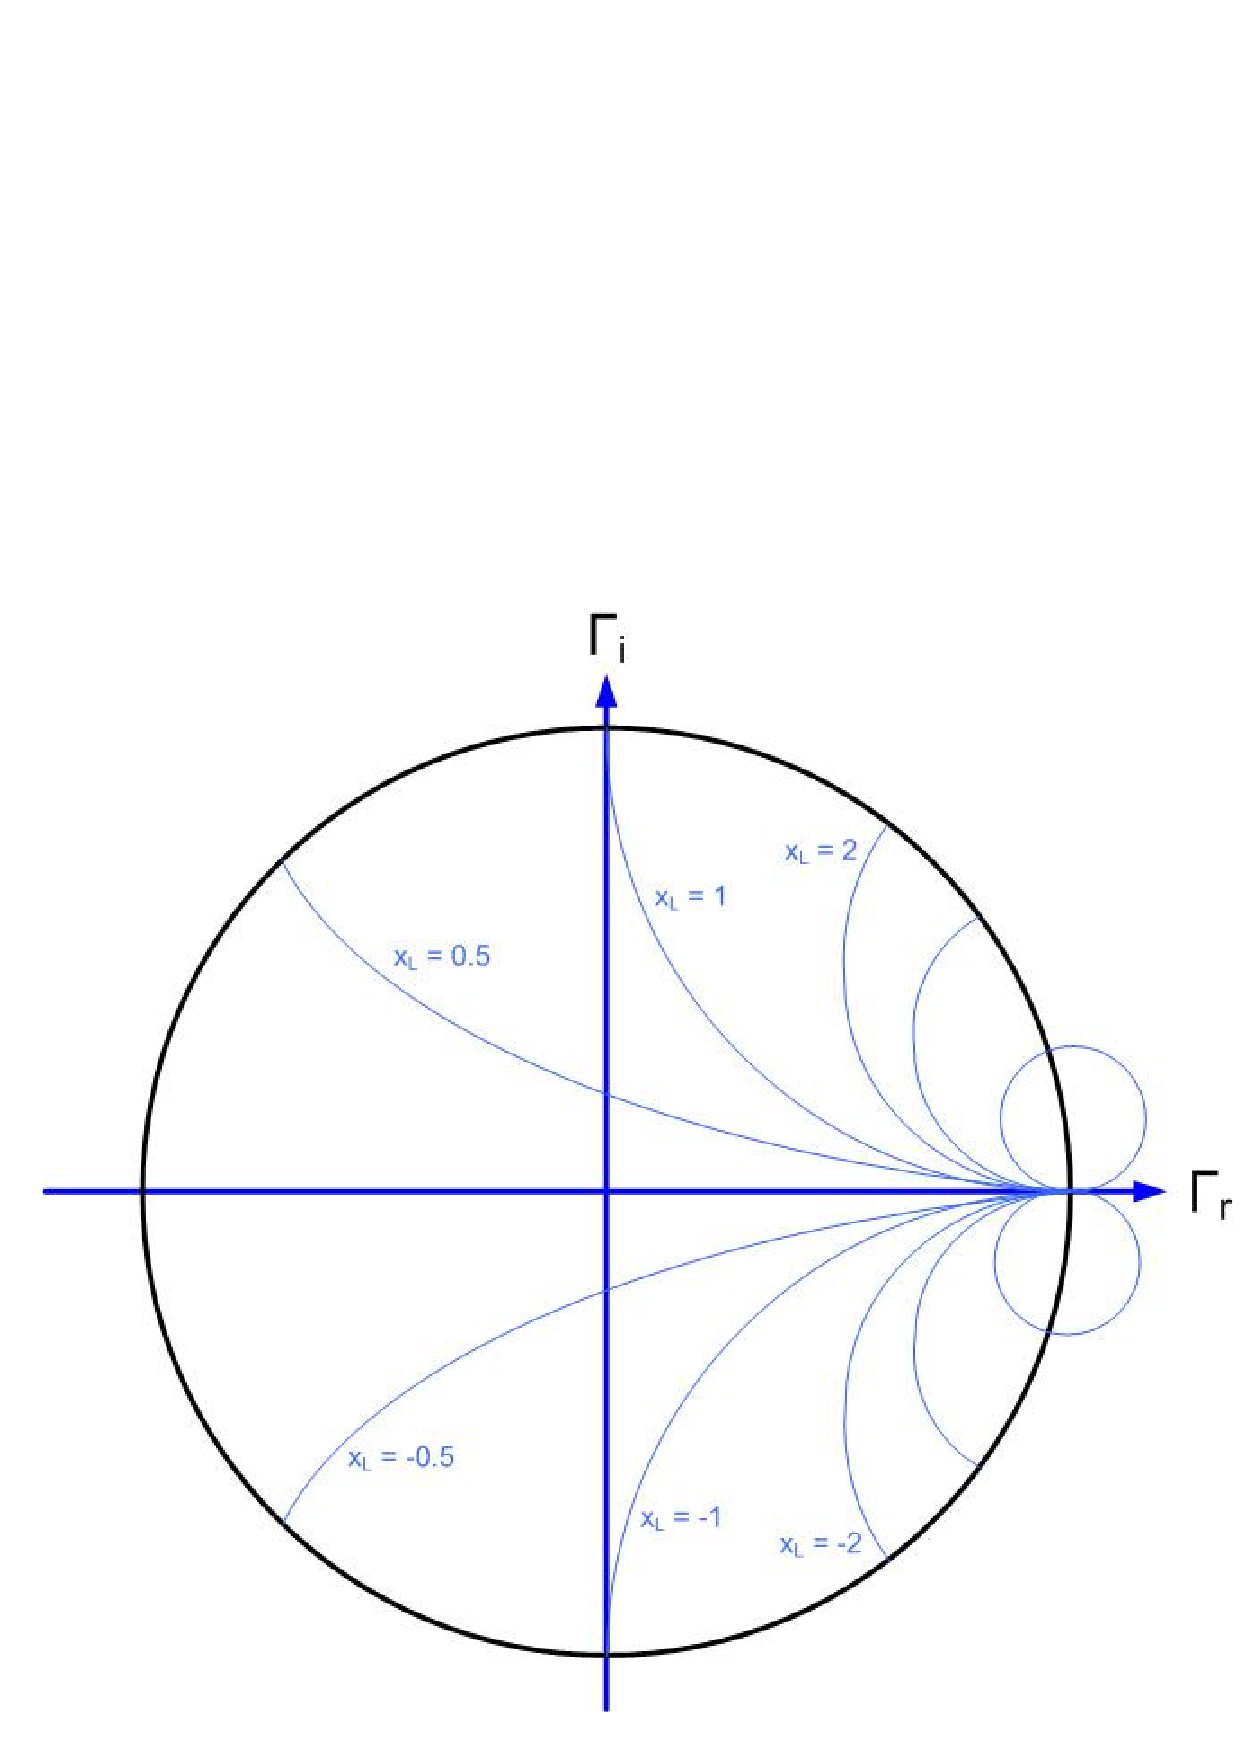
\includegraphics[scale=0.3]{../jpg/smithchartimaginary.jpg}
\end{center}
\caption{All points on the circle have the constant imaginary part of the impedance (reactance). Normalized reactance circles.}
\label{fig:SCDerscreactance}
\end{figure}

Admittance circles can be similarly derived using the fact that $Y_L=\frac{1}{Z_L}$ and the Equation \ref{eq:SCDerNormImp}


\end{document} 
